\documentclass[12pt,twoside,a4paper]{article}
\usepackage[utf8]{inputenc} \usepackage[T1]{fontenc} \usepackage{graphicx} \usepackage{underscore}
\setlength\parindent{0pt} 
\author{Thorben Schomacker}
\author{Ferdinand Trendelenburg}
\begin{document}

\part*{Lösung Ü3, Gruppe C}

\section{EA3.2}

Sobald ein ER kommt wird ein X ausgegeben, bei SIE ein Y und bei ES ein Z. 
Es können beliebig viele Buchstaben eingeben werden, alle Buchstabenkombinationen außer ER, SIE, ES werden überlesen.

\begin{figure}[!htb]
\centering
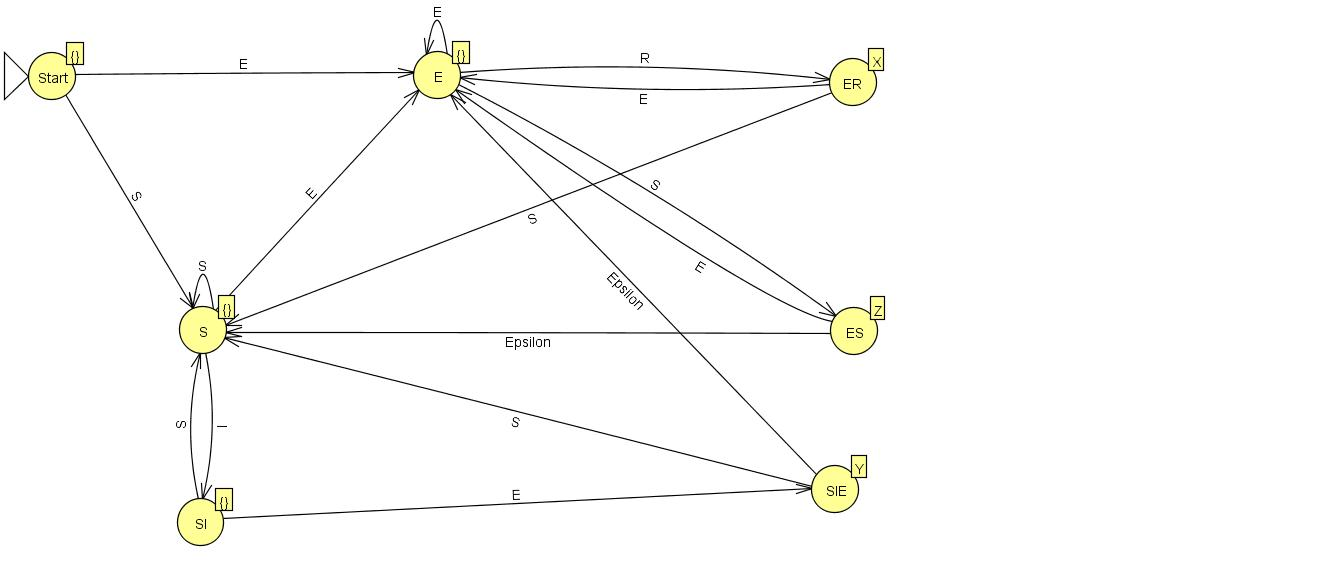
\includegraphics[width=180mm]{32moore.jpg}
\caption{Moore \label{overflow}}
\end{figure}

\begin{figure}[!htb]
\centering
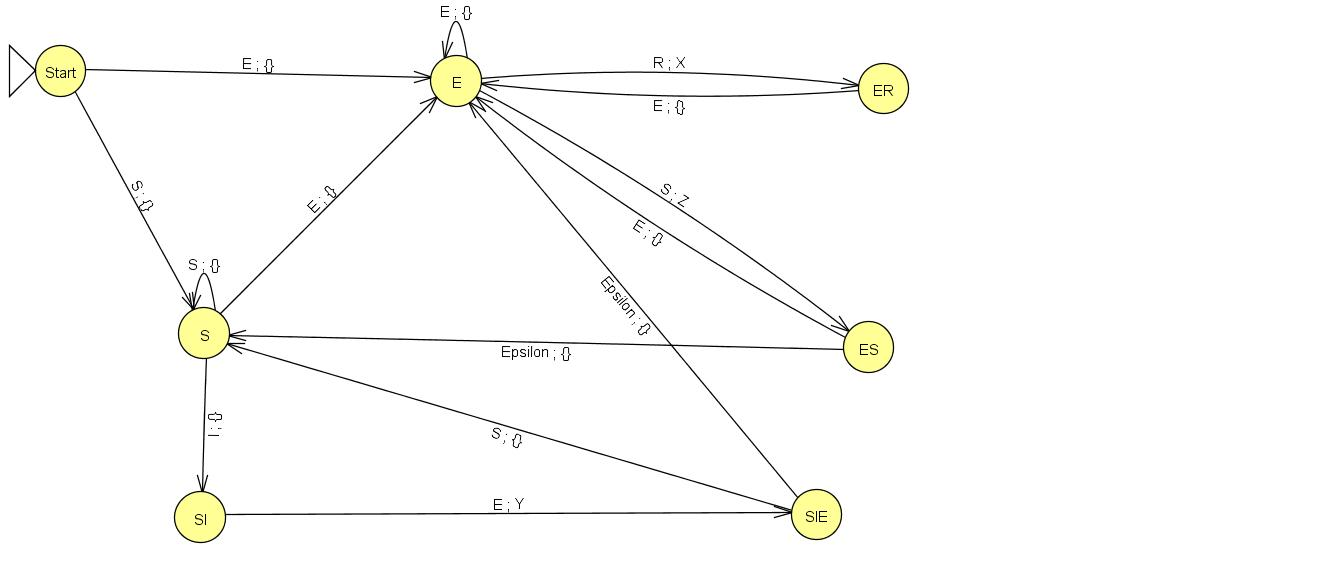
\includegraphics[width=180mm]{32mealy.jpg}
\caption{Mealy \label{overflow}}
\end{figure}

\newpage 
\section{EA3.3}

Merkmale der Sprache: Es werden immer Pärchen aus 0en, 1en und einem Übertrag ausgewertet. Es wird von rechts nach links gelesen.Die Möglichkeiten sind: \\
Input 00 Übertrag 0 = Ergebnis 0, Übertrag 0 \\
Input 01 Übertrag 0 = Ergebnis 1, Übertrag 0 \\
Input 10 Übertrag 0 = Ergebnis 1, Übertrag 0 \\
Input 11 Übertrag 0 = Ergebnis 0, Übertrag 1 \\

Input 00 Übertrag 1 = Ergebnis 1, Übertrag 0 \\
Input 01 Übertrag 1 = Ergebnis 0, Übertrag 1 \\
Input 10 Übertrag 1 = Ergebnis 0, Übertrag 1 \\
Input 11 Übertrag 1 = Ergebnis 1, Übertrag 1 \\

\begin{figure}[!htb]
\centering
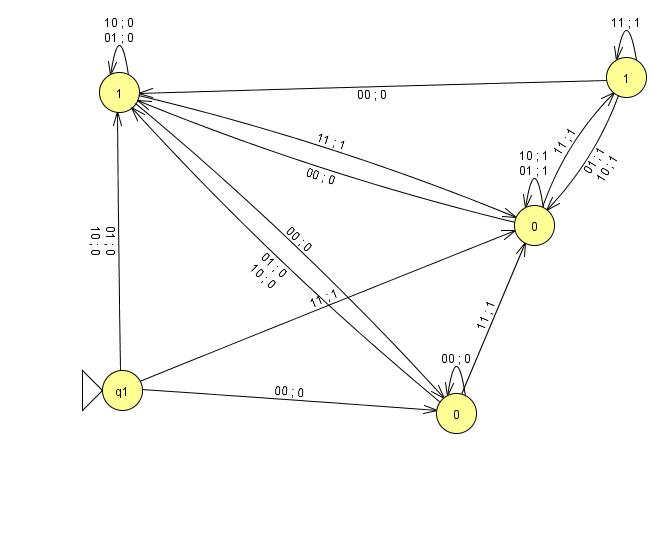
\includegraphics[width=180mm]{33moore.jpg}
\caption{Moore \label{overflow}}
\end{figure}


\end{document}